\begin{evenBlock}{3v2+Keeper}

\begin{minipage}[t]{\linewidth}
    \centering
    
    \begin{minipage}{.5\linewidth} % Left column and width
        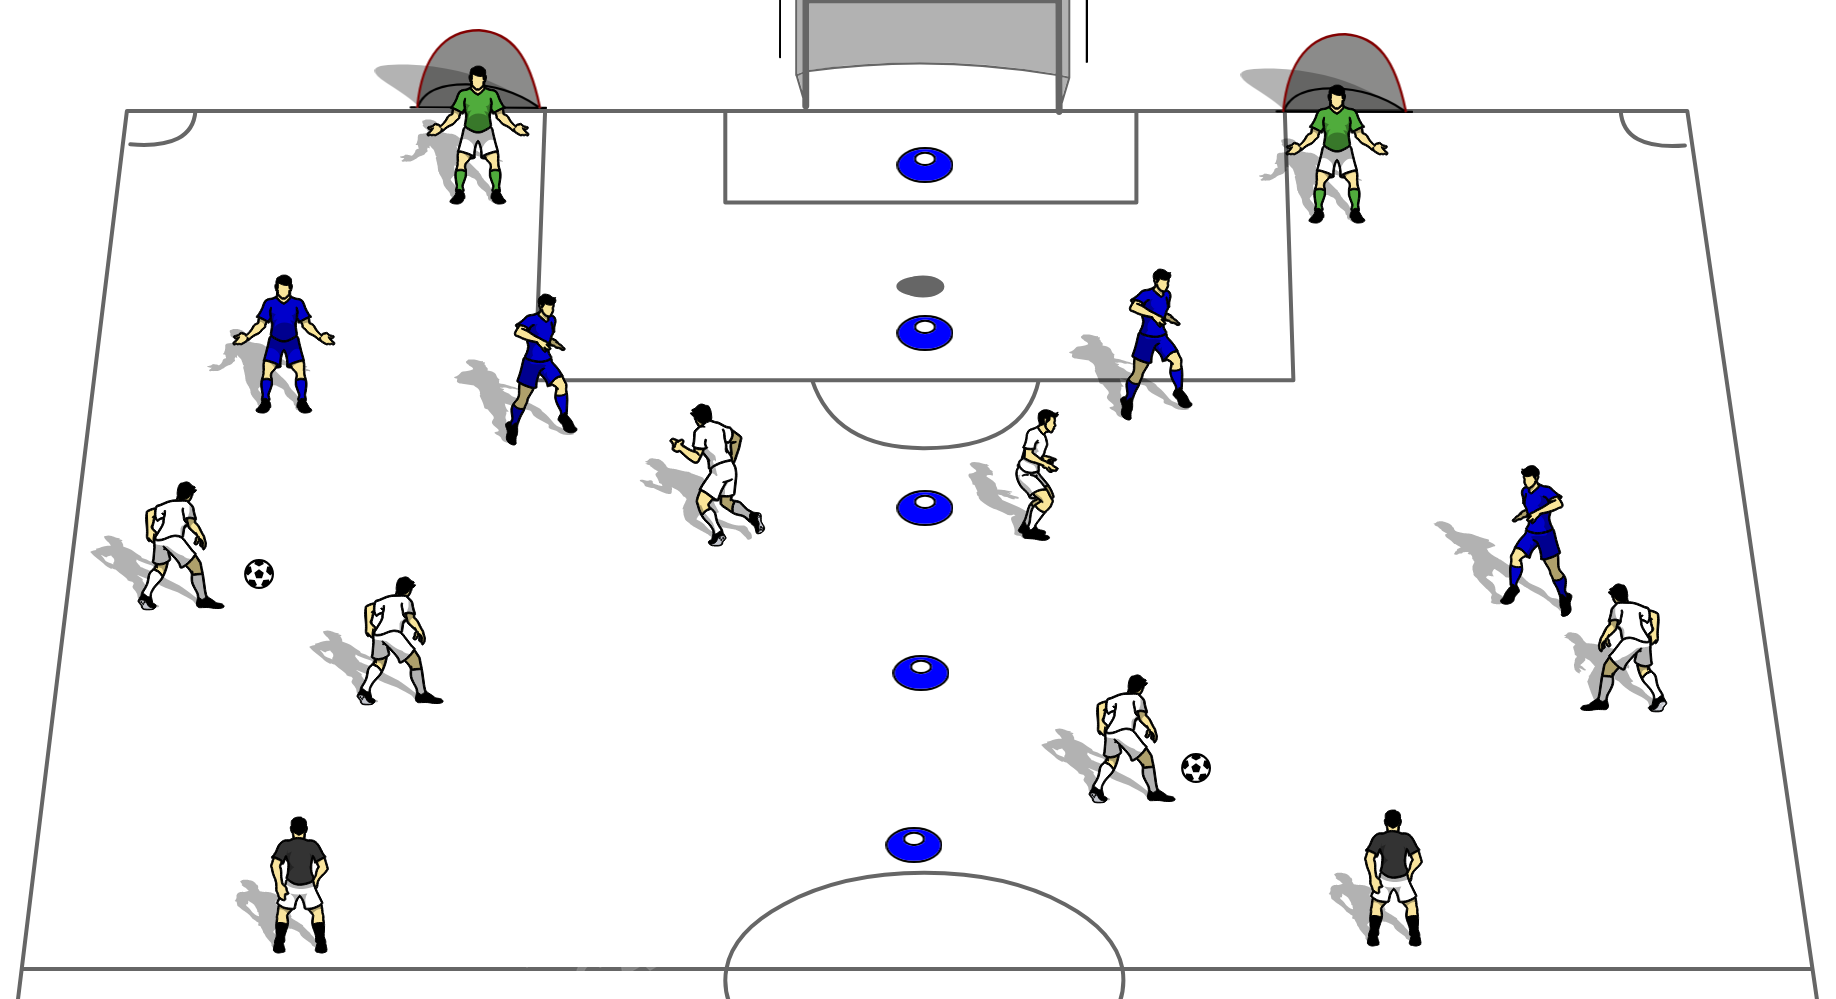
\includegraphics[width=\textwidth]{../img/Trimmed/3v2+Keeper}
    \end{minipage}
    \hspace{0.05\linewidth}
    \begin{minipage}{.4\linewidth} % Left column and width
        \textbf{Drill Description:}
        This drill requires 6 players + 1 coach or 12 players and 2 coaches.
        \begin{enumerate}
            \setlength{\itemsep}{0pt}
            \setlength{\parskip}{0pt}
            \setlength{\parsep}{0pt}
            \item The defending team uses 2 defenders and 1 keeper.
            \item Attacking team has 3 and tries to score on the small defended goal.
            \item The defending team scores by completing a pass to the coach on the center line.
        \end{enumerate}
    \end{minipage}
\end{minipage}
\vspace{12pt}

\textbf{Coaching Points:}
\begin{itemize}
    \setlength{\itemsep}{0pt}
    \setlength{\parskip}{0pt}
    \setlength{\parsep}{0pt}
    \item Explain marking a player is to remain within 2 or 3 feet of the attacking player.
    \item Explain how to mark a player goal side (defender between the attacker and goal).
    \item Attackers try to lose their marks by passing.
\end{itemize}
\end{evenBlock}